\section{Er-Mapping 1}
Address: \underline{address\_id}, street, number, zip\_code, city, state\\
Customer: \underline{customer\_id} creation\_date\\
PrivatePerson: \dashuline{\underline{customer\_id}}, fristname, lastname, birthday \\
Buisness: \dashuline{\underline{customer\_id}}, name, telephone\_number \\
Order: \underline{order\_id}, order\_date, delivery\_date \\ 
Computer: \underline{serial\_no} \\
Software: \underline{name}, \underline{version}, description \\
OS: \underline{name}, \underline{version}, description \\

\begin{minipage}{0.5\textwidth}
        \centering
        \begin{tabular}{|c|c|c|c|c|c|}
            \hline
            \multicolumn{6}{|c|}{Address}\\
            \hline
            \underline{address\_id} & street & number & zip\_code & city & state \\
            \hline
        \end{tabular}
\end{minipage}
\begin{minipage}{0.5\textwidth}
    \centering
        \begin{tabular}{|c|c|}
            \hline
            \multicolumn{2}{|c|}{Customer}\\
            \hline
            \underline{customer\_id} & creation\_date \\
            \hline
        \end{tabular}
\end{minipage}
\vspace{20px}

\begin{minipage}{0.5\textwidth}
    \centering
    \begin{tabular}{|c|c|c|c|}
        \hline
        \multicolumn{4}{|c|}{PrivatePerson}\\
        \hline
        \dashuline{\underline{customer\_id}} & firstname & lastname & birthday \\
        \hline
    \end{tabular}
\end{minipage}
\begin{minipage}{0.5\textwidth}
    \centering
    \begin{tabular}{|c|c|c|}
        \hline
        \multicolumn{3}{|c|}{Buisness}\\
        \hline
        \dashuline{\underline{customer\_id}} & name & telephone\_number \\
        \hline
    \end{tabular}
\end{minipage}

\vspace{20px}

\begin{minipage}{0.5\textwidth}
    \centering
    \begin{tabular}{|c|c|c|}
        \hline
        \multicolumn{3}{|c|}{Order}\\
        \hline
        \underline{order\_id} & order\_date & delivery\_date \\
        \hline
    \end{tabular}
\end{minipage}
\begin{minipage}{0.5\textwidth}
    \centering
    \begin{tabular}{|c|}
        \hline
        \multicolumn{1}{|c|}{Computer}\\
        \hline
        \underline{serial\_no}\\
        \hline
    \end{tabular}
\end{minipage}

\vspace{20px}
\begin{minipage}{0.5\textwidth}
    \centering
    \begin{tabular}{|c|c|c|}
        \hline
        \multicolumn{3}{|c|}{Softare}\\
        \hline
        \underline{name} & \underline{version} & description\\
        \hline
    \end{tabular}
\end{minipage}
\begin{minipage}{0.5\textwidth}
    \centering
    \begin{tabular}{|c|c|c|}
        \hline
        \multicolumn{3}{|c|}{OS}\\
        \hline
        \underline{name} & \underline{version} & description\\
        \hline
    \end{tabular}
\end{minipage}



\newpage
\section{Er-Mapping 2}
User: \underline{user\_id}, username, email, description, data\_registered, noWrittenTexts \\
follows: \dashuline{\underline{user\_id}}, timestamp \\
Test: \underline{text\_id}, timestamp, text \\


\newpage
\section{Er-Daigramm}
    \begin{figure}[!htb]
        \centering
        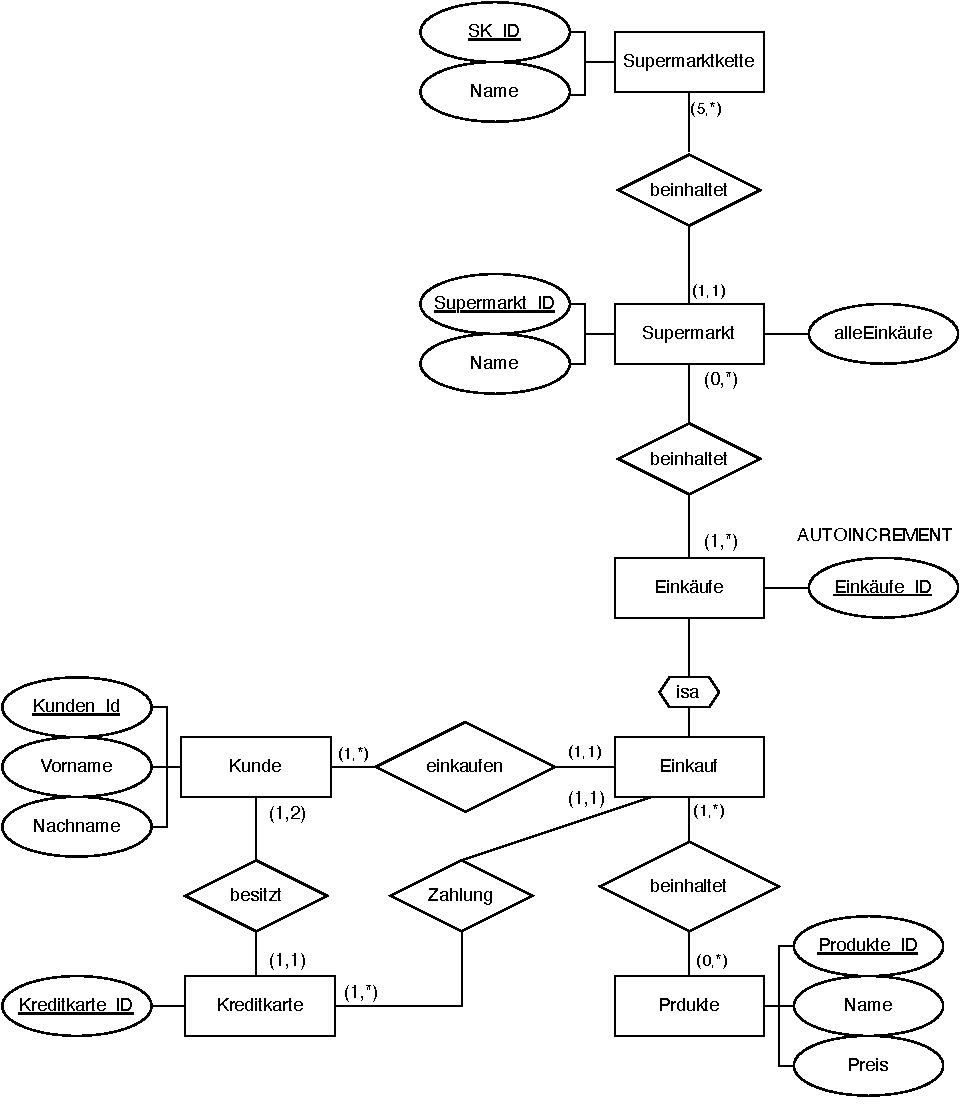
\includegraphics[scale=1]{ER.pdf}
        \caption{ER-Diagramm-Supermarktkette}
        \label{caption:ER-Diagramm-Supermarktkette}
    \end{figure}
    

\newpage{}
\section{ER-Mapping 3}
Kunden: \underline{Kunden\_ID}, Vorname, Nachname \\
Kreditkarte: \underline{Kreditkarder\_ID} \\
Einkauf: \dashuline{\underline{Einkäufe\_ID}}, Uhrzeit \\
Produkte: \underline{Produkt\_ID}, Name, Preis \\
Einkäufe: \underline{Einkäufe\_ID} \\
Supermarkt: \underline{Supermarkt\_ID}, Name, alleEinkäufe \\ 
Supermarktkette: \underline{Supermarktkette\_ID}, Name

